\section{Quality versus output budget}
\label{app:quality}

At output budget 128, dense AR-3B retains
\arFOneTwentyEight{} 9-field F1 and \arValidTwentyEight\%
schema validity, while DG has \dgFOneTwentyEight{} and
\dgValidTwentyEight\%. Thus a small budget can prevent usable DG
records even when the cost model predicts low latency. This experiment
varies the allowed output budget, not the native canvas-size setting.

\begin{figure}[ht!]
\centering
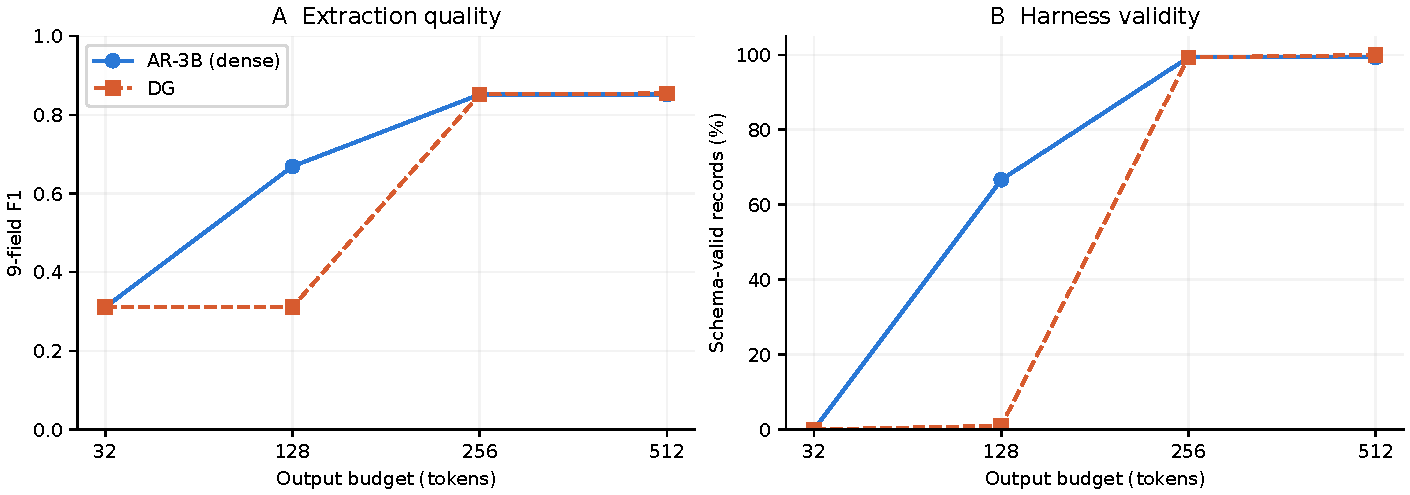
\includegraphics[width=\linewidth]{figures/fig5_quality_vs_length.pdf}
\caption{Quality and schema validity versus constrained output budget
(BGL, $n{=}300$; dense AR-3B baseline). DG improves sharply once the
budget permits a complete record. First-object-wins parsing keeps AR-3B
F1 stable from budgets 256 to 512 despite repeated continuations.
Neither curve constitutes a guarantee of valid output.}
\label{fig:quality}
\end{figure}

Lowering $K$ is a distinct intervention and can trade quality for service
time without reducing the nominal token budget. Its value must still be
assessed using observed validity and correctness; a denoised token canvas
can contain malformed or incorrect JSON.
